\documentclass[a4paper,14pt]{extreport}
\usepackage[left=1.5cm,right=1.5cm,
    top=1.5cm,bottom=2cm,bindingoffset=0cm]{geometry}
\usepackage{scrextend}
\usepackage[T1,T2A]{fontenc}
\usepackage[utf8]{inputenc}
\usepackage[english,russian,ukrainian]{babel}
\usepackage{tabularx}
\usepackage{amssymb}
\usepackage{color}
\usepackage{amsmath}
\usepackage{mathrsfs}
\usepackage{listings}
\usepackage{graphicx}
\graphicspath{ {./images/} }
\usepackage{lipsum}
\usepackage{xcolor}
\usepackage{hyperref}
\usepackage{tcolorbox}
\usepackage{tikz}
\usepackage[framemethod=TikZ]{mdframed}
\usepackage{wrapfig,boxedminipage,lipsum}
\mdfdefinestyle{MyFrame}{%
linecolor=blue,outerlinewidth=2pt,roundcorner=20pt,innertopmargin=\baselineskip,innerbottommargin=\baselineskip,innerrightmargin=20pt,innerleftmargin=20pt,backgroundcolor=gray!50!white}
 \usepackage{csvsimple}
 \usepackage{supertabular}
\usepackage{pdflscape}
\usepackage{fancyvrb}
%\usepackage{comment}
\usepackage{array,tabularx}
\usepackage{colortbl}

\usepackage{varwidth}
\tcbuselibrary{skins}
\usepackage{fancybox}


\usepackage{tikz}
\usepackage[framemethod=TikZ]{mdframed}
\usepackage{xcolor}
\usetikzlibrary{calc}
\makeatletter
\newlength{\mylength}
\xdef\CircleFactor{1.1}
\setlength\mylength{\dimexpr\f@size pt}
\newsavebox{\mybox}
\newcommand*\circled[2][draw=blue]{\savebox\mybox{\vbox{\vphantom{WL1/}#1}}\setlength\mylength{\dimexpr\CircleFactor\dimexpr\ht\mybox+\dp\mybox\relax\relax}\tikzset{mystyle/.style={circle,#1,minimum height={\mylength}}}
\tikz[baseline=(char.base)]
\node[mystyle] (char) {#2};}
\makeatother

\definecolor{ggreen}{rgb}{0.4,1,0}
\definecolor{rred}{rgb}{1,0.1,0.1}
\definecolor{amber}{rgb}{1.0, 0.75, 0.0}
\definecolor{babyblue}{rgb}{0.54, 0.81, 0.94}
\definecolor{asparagus}{rgb}{0.53, 0.66, 0.42}
\definecolor{chartreuse}{rgb}{0.5, 1.0, 0.0}
\definecolor{darkorchid}{rgb}{0.6, 0.2, 0.8}

\usepackage{float}
\usepackage{wrapfig}
\usepackage{framed}
%for nice Code{
\lstdefinestyle{customc}{
  belowcaptionskip=1\baselineskip,
  breaklines=true,
  frame=L,
  xleftmargin=\parindent,
  language=C,
  showstringspaces=false,
  basicstyle=\small\ttfamily,
  keywordstyle=\bfseries\color{green!40!black},
  commentstyle=\itshape\color{purple!40!black},
  identifierstyle=\color{blue},
  stringstyle=\color{orange},
}
\lstset{escapechar=@,style=customc}
%}


\begin{document}
\pagecolor{white}

%----------------------------------------1
\newtcbox{\xmybox}[1][red]{on line, arc=7pt,colback=#1!10!white,colframe=#1!50!black, before upper={\rule[3pt] {0pt}{10pt}},boxrule=1pt,boxsep=0pt,left=6pt,right=6pt,top=2pt,bottom=2pt}

\begin{center}\xmybox[amber]{Mnatsakanov Anton} \xmybox[amber]{DP-82}
\vspace{1cm}

\xmybox[darkorchid]{Індивідуальне тестове завдання вар. № 54}
\end{center}

\xmybox[ggreen]{1}. Які основні домішки, використовують для створення шарів з акцепторною провідністю?\par
Матеріали, що складаються з елементів IV групи таблиці Менделєєва, акцепторами елементів Кремнію та Германію є елементи III, тобто це Бор, Індій, Алюміній, Титан, Галій.\\
\xmybox[ggreen]{2}. Інтегральна цифрова мікросхема має $10^7$ елементів. Визначити ступень інтеграції мікросхеми.\par
ІМС 7 ступеню інтеграції. Надвелика ІМС.\\
\xmybox[ggreen]{3}. Який шар біполярного транзистора має максимальну ступінь легування?\par
Емітерний, до 1021 см$^{-3}$\\
\xmybox[ggreen]{4}. Накресліть поперечний розріз епітаксіального планарного біполярного транзистора з ізоляцією р – п переходом .\par
\begin{figure}[h!]
\center{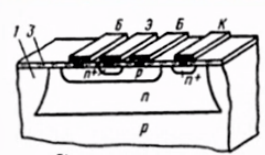
\includegraphics[width=0.4\linewidth]{1.png}}
\end{figure}
\begin{figure}[h!]
\xmybox[ggreen]{5}. Показати п’ять можливих схем діодного включення біполярного транзистора.\par
\center{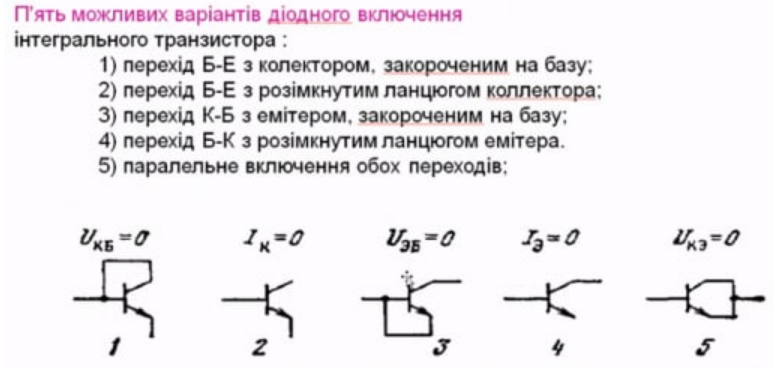
\includegraphics[width=0.8\linewidth]{4.png}}
\end{figure}


\xmybox[ggreen]{6}. Для чого використовують в планарно – епітаксіальних біполярних n-p-n транзисторах ІС прихований n+ шар?\par
Для зменшення опору колекторної області.\\
\xmybox[ggreen]{7}. Який тип транзисторів в інтегральних схемах є основним — n-p-n чи p-n-p тип, і чому?\par
 n-p-n, тому що рухливість електронів більша за рухливість дірок.\\
\xmybox[ggreen]{8}. Визначити коефіцієнти підсилення по струму в схемі із загальним емітером, коли значення коефіцієнти підсилення по струму в схемі із загальною базою дорівнює 0,992.\par
$\beta = \dfrac{\alpha}{1-\alpha} = 124$\\
\xmybox[ggreen]{9}. Накресліть еквівалентну схему інтегрального біполярного п-р-п транзистора.\par
\begin{figure}[h!]
\xmybox[ggreen]{10}. Накресліть розподіл концентрацій домішок в структурі інтегрального планарно - епітаксіального біполярного п-р-п транзистора.\par



\center{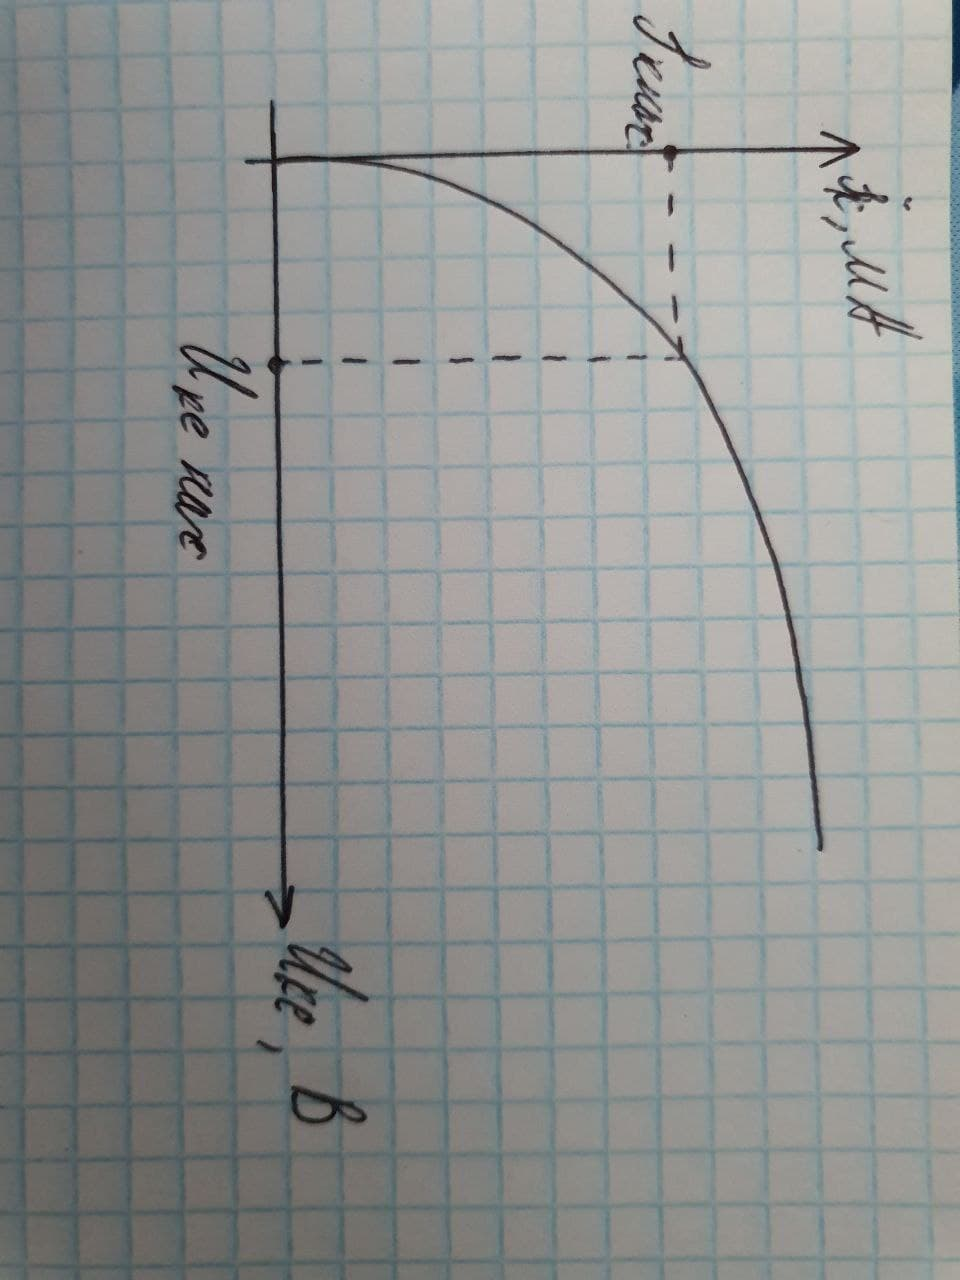
\includegraphics[angle = 90, width=0.3\linewidth]{2.jpg}}
\end{figure}
\begin{figure}[h!]
\xmybox[ggreen]{11}. Представити вихідні характеристики в схемі з загальним емітером для біполярних транзисторів в ІС з прихованим n + шаром та без прихованого
n + шару.\par

\center{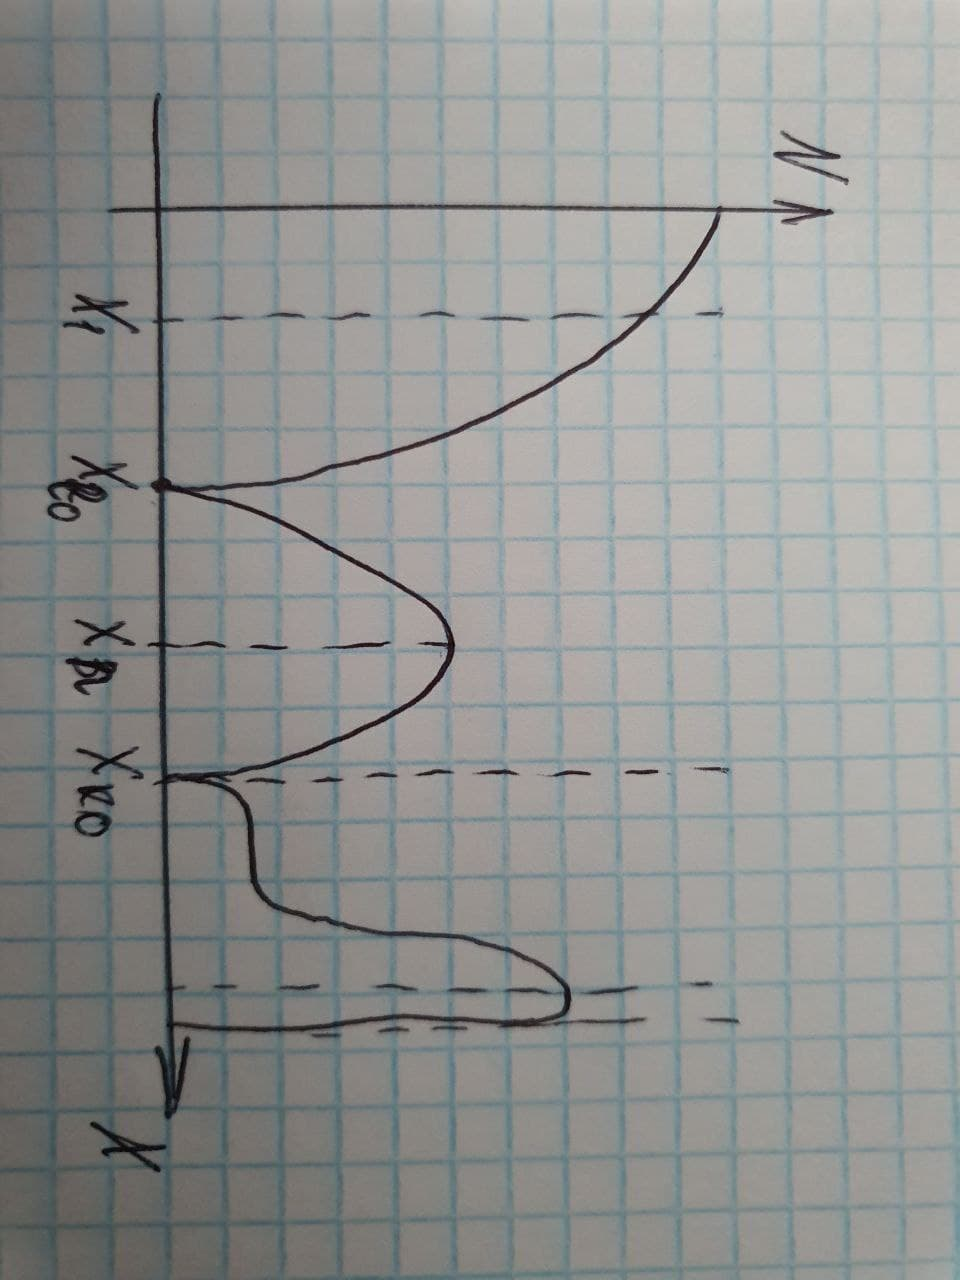
\includegraphics[angle = 90,width=0.3\linewidth]{3.jpg}}
\end{figure}

\end{document}
